% ------------------------------------------------------------
% DO NOT CHANGE: BEGIN
% ------------------------------------------------------------

\documentclass [a4paper, 11pt] {article}


\usepackage[utf8]{inputenc}  
\usepackage[T1]{fontenc}  
\usepackage{lmodern}
\usepackage[english]{babel}
\usepackage{fancybox}
\usepackage{listings}
\usepackage{color}
\usepackage{graphicx,subfigure}
\usepackage[titletoc]{appendix}
\usepackage{float} % figures flottantes 
\usepackage{here} % figures flottantes
\usepackage{url}
\usepackage{enumitem}
\setlist[itemize]{noitemsep, nolistsep}
\setlist[enumerate]{noitemsep, nolistsep}
\usepackage{xcolor}
\usepackage[colorlinks=false]{hyperref}
\usepackage{tabularx}
\usepackage{amsmath}
\usepackage[skins,breakable]{tcolorbox}
\usepackage{lipsum}  


% --------------------------------------------------------------
% Title
% --------------------------------------------------------------
\makeatletter
\newcommand\maintitle[1]{
    \quitvmode
    \hb@xt@\linewidth{
        \dimen@=1ex
        \advance\dimen@-2pt
        \leaders\hrule \@height1ex \@depth-\dimen@\hfill
        \enskip
        \textbf{#1}
        \enskip
        \leaders\hrule \@height1ex \@depth-\dimen@\hfill
    }
}
\makeatother

% --------------------------------------------------------------
% Some parameters
% --------------------------------------------------------------
\oddsidemargin =0 mm
\topmargin = -15 mm
\footskip = 20mm
\textheight = 260 mm 
\textwidth = 160mm

% --------------------------------------------------------------
% Q&A environments
% --------------------------------------------------------------

\usepackage{tikz}

\newcommand{\emptyquestion}{Please fill this space with your question.}

\newcommand{\emptyanswer}{Please fill this space with your answer.}

\newcounter{question}

\definecolor{question_color}{RGB}{7,128,164}
\definecolor{question_color_fill}{RGB}{247,247,247}

\newcommand{\thequestionref}{No reference}

\makeatletter
\newenvironment{question}[1]
{
\refstepcounter{question}
\def\@currentlabel{{#1}}
\label{ref-question-\thequestion}
\addcontentsline{toc}{subsection}{{#1}}
\noindent
\begin{tcolorbox}[
    colframe=question_color,
    colback=question_color_fill,
    coltitle=question_color_fill,  
    title=\centering\textbf{Question #1},
    breakable,
    width=\textwidth]
}
{   \end{tcolorbox}
}
\makeatother




\newenvironment{answer}[1]
{
\def\L{#1}
\noindent
{
\hypersetup{allcolors=question_color}
\flushleft
\begin{tikzpicture}
	
    \draw[very thick,question_color] (0,0) -- ++(0,+7.5pt)
    -- ++(\textwidth,0) node[midway,above] {\textbf{Answer to \ref{ref-question-\thequestion}}}
    -- ++(0,-7.5pt);
    
    
    \begin{scope}[yshift =-\L cm]
     \draw[very thick,question_color] (0,0) -- ++(0,-7.5pt)
    -- ++(\textwidth,0)
    -- ++(0,+7.5pt);
    \end{scope}
    
\end{tikzpicture}

\vspace{-\L cm}
}
\begin{tcolorbox}[blanker,width=\textwidth, height=1cm, bottom=5pt]}
{   \end{tcolorbox}
\vspace{\L cm}
\flushleft
}

\begin{document}

    \begin{center}
        \Large
        \centering
        \maintitle{LEPL1109 - Statistics and Data Sciences}
        \textsc{\textbf{HACKATHON 2 - Classification: Stars, Galaxies and Quasars}}\\
    	\vspace{0.3cm}
         \hfill Deadline: December 4, 2023 \\
       \noindent\hrulefill
    \end{center}
    \vspace*{0.5cm}

% ------------------------------------------------------------
% DO NOT CHANGE: END
% ------------------------------------------------------------


% ------------------------------------------------------------
% FILL WITH YOUR NAMES: BEGIN
% ------------------------------------------------------------
    \hspace*{-0.75cm}
    \fbox{\parbox{\textwidth}{
    \begin{tabularx}{\textwidth}{X|X|{c}p{2cm}}
       \textbf{Lastname}  & \textbf{Firstname} & \textbf{Noma} \\
       \hline
        <Lastname 1> & <Firstname 1> & 12345678 \\
        <Lastname 2> & <Firstname 2> & 12345678 \\
        <Lastname 3> & <Firstname 3> & 12345678 \\
        <Lastname 4> & <Firstname 4> & 12345678 \\
    \end{tabularx}
    }}
% ------------------------------------------------------------
% FILL WITH YOUR NAMES: END
% ------------------------------------------------------------

% ------------------------------------------------------------
% DO NOT CHANGE: BEGIN
% ------------------------------------------------------------

    \vspace*{2.5cm}
    
    \hrule
    
    \vspace*{0.5cm}
    
    Please, read carefully the following guidelines:
    \vspace*{0.2cm}
    \begin{itemize}
        \item Answer in English or French.
        \item \textbf{Do not modify the layout of the document.} Tour answers will be imported into gradescope for correction. Each answer must be contained in the "zone" predefined by the template.
        \item Clearly cite every source of information (even for pictures!);
        \item Whenever possible, use the \texttt{.pdf} format when you export your images: this usually makes your report look prettier\footnote{This is because \texttt{.pdf} is a vector format, meaning that it keeps a perfect description of your image, while \texttt{.png} and other standard formats use compression. In other words, this means you can zoom as much as you want on your figure without decreasing image resolution. For simple plots, vector formats can also save a lot of memory space. On the other hand, we recommend using \texttt{.png} when you are plotting many data points: large scatter plots, heatmap, etc.};
        \item Do not forget to also submit your code on Moodle.
    \end{itemize}
    
    \vspace*{0.5cm}
    
      \hrule
   	
   	\vspace*{2.0cm}   
      
\begin{minipage}{0.5\textwidth}
\centering
	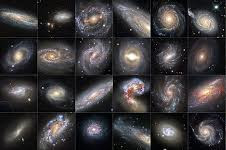
\includegraphics[width=0.9\textwidth]{imgs/stellar.jpeg}
	Image source \cite{StellarImg}.
\end{minipage}%
\begin{minipage}{0.45\textwidth}
The dataset \cite{carvalho_2022} consists of 100,000 observations of space taken by the SDSS (Sloan Digital Sky Survey). Every observation is described by 17 feature columns and 1 class column which identifies it to be either a star, galaxy or quasar.\\

The project aims at building a ternary classifier for the following 3 classes: star, galaxy or quasar. 
\end{minipage}

    {
    \hypersetup{allcolors=black}
    }
    \newpage
    % -----------------------------------------------------------------------
% Question 1.1
% -----------------------------------------------------------------------

\begin{question}{1.1}
Describe, briefly, your dataset (size, variables type, missing values, etc.).
\end{question}
\begin{answer}{3} 
    Your answer to question 1.1 in this box.
\end{answer}

% -----------------------------------------------------------------------
% Question 1.2
% -----------------------------------------------------------------------

\begin{question}{1.2}
Based on a study of the features distribution (variance, number of unique values, number of missing values, etc.), can you identify some features that do not provide useful information for the classification task? Explain your analysis and remove those features from the dataset. 
\end{question}
\begin{answer}{11} 
    Your answer to question 1.2 in this box.
\end{answer}


% -----------------------------------------------------------------------
% Question 1.3
% -----------------------------------------------------------------------

\begin{question}{1.3}
What are the drawbacks (if any) of choosing a small test set (in proportion)? On the contrary, what are the consequences (if any) of a relatively large testing set (in proportion)?
\end{question}

\begin{answer}{7} 
    Your answer to question 1.3 in this box.
\end{answer}

    \pagebreak
    % -----------------------------------------------------------------------
% Question 2.1
% -----------------------------------------------------------------------

\begin{question}{2.1}
Are the ternary classes balanced? What are the proportions of data in each class? Briefly, justify your answer and add a visualization. 
\end{question}

\begin{answer}{11} 
    Your answer to question 2.1 in this box.
\end{answer}




% -----------------------------------------------------------------------
% Question 2.2
% -----------------------------------------------------------------------

\begin{question}{2.2}
What would be the expected performance of a random classifier on this dataset? 
\end{question}

\begin{answer}{3} 
    Your answer to question 2.2 in this box.
\end{answer}


% -----------------------------------------------------------------------
% Question 2.3
% -----------------------------------------------------------------------

\begin{question}{2.3}
Compute the correlation matrix of the dataset and plot it. Do you want to discard features based on this observation?
Write clearly you decision rule. 
\end{question}

\begin{answer}{19} 
    Your answer to question 2.3 in this box.
\end{answer}


% -----------------------------------------------------------------------
% Question 2.4
% -----------------------------------------------------------------------

\begin{question}{2.4}
 Why do we scale data? Justify properly, whether it is necessary or not for your feature set (X) and which scaler did you use. 
\end{question}

\begin{answer}{8} 
    Your answer to question 2.3 in this box.
\end{answer}


    \pagebreak
    % -----------------------------------------------------------------------
% Question 3.1
% -----------------------------------------------------------------------

\begin{question}{3.1}
Explain the idea of K-fold cross-validation and why it is useful. How the choice of K (in the cross-validation) impacts the bias and the variance of the scores obtained on the different folds? Choose and justify the number of folds you consider in this project. 
\end{question}

\begin{answer}{12} 
    Your answer to question 2.1 in this box.
\end{answer}



% -----------------------------------------------------------------------
% Question 3.2
% -----------------------------------------------------------------------

\begin{question}{3.2}
Explain your methodology of model evaluation. More precisely, explain which hyperparameters you tune and the values you test for each of them. Next, provide the best hyperparameters configuration for each of the three models as well as their CV F1 score. 
\end{question}

\begin{answer}{13} 
    Your answer to question 3.2 in this box.
\end{answer}



% -----------------------------------------------------------------------
% Question 3.3
% -----------------------------------------------------------------------

\begin{question}{3.3}
Based on your answers to previous questions, select a final model that you will keep as classifier. Justify. 
\end{question}

\begin{answer}{4} 
    Your answer to question 3.3 in this box.
\end{answer}


% -----------------------------------------------------------------------
% Question 3.4
% -----------------------------------------------------------------------

\begin{question}{3.4}
Plot the precision-recall curve for the three methods, one figure for each class. What happens to the precision and recall when the threshold tends to 0? And when it tends to 1? Explain and, if possible, establish a link with Question 2.1.
For each class, for each method: what threshold would you use?  
\end{question}

\begin{answer}{18} 
    Your answer to question 3.4 in this box.
\end{answer}

    \pagebreak
    % -----------------------------------------------------------------------
% Question 4.1
% -----------------------------------------------------------------------

\begin{question}{4.1}
Use the test set to estimate the precision, recall and F1 score of your final model and validate its performance on unseen data.
Observe if the scores are similar to the ones estimated with your cross-validation. Are you satisfied by the performance of your classifier, in view of the task for which it will be used? 
\end{question}

\begin{answer}{12} 
    Your answer to question 4.1 in this box.
\end{answer}



        
    \pagebreak
    \addcontentsline{toc}{section}{References}
    \bibliographystyle{unsrt}
    \bibliography{biblio}


\end{document}

% ------------------------------------------------------------
% DO NOT CHANGE: END
% ------------------------------------------------------------